\documentclass[UTF8]{article}

\usepackage{ctex}
\usepackage{fancyhdr} %自定义页眉页脚
\usepackage{listings} %source code
\usepackage{tabu}
\usepackage{booktabs}
\usepackage{graphicx}
\usepackage{multirow}
\usepackage[colorlinks,linkcolor=blue]{hyperref}
\usepackage{subfigure}
\usepackage{float}
\begin{document}


\begin{titlepage}
\center{北京理工大学计算机学院2017级}
\vspace{2cm}
\center{\huge{《数字逻辑》实验三  实验报告}}
\vspace{0.5cm}
\center{\Huge{单周期CPU设计}}
\vspace{2cm}

\begin{center}
\begin{large}
\begin{tabular}{c c |c c}
小组编号& 44 & 指导老师 & 王娟\\
\cline{2-2} \cline{4-4}
\hline
学\qquad 号& 1120173323 & 电\qquad 话& 592175501@qq.com \\
\cline{2-2} \cline{4-4}
姓\qquad 名& 王聚海 & 邮\qquad 箱& 13521592752 \\
\cline{2-2} \cline{4-4}
班\qquad 级 & 07111703 \\
\cline{2-2}
\hline
学\qquad 号& 1120171224 \\
\cline{2-2}
姓\qquad 名& 冯开宇 \\
\cline{2-2}
班\qquad 级 & 07111701 \\
\cline{2-2}
\hline
学\qquad 号& 1120172200 \\
\cline{2-2}
姓\qquad 名& 刘思雨 \\
\cline{2-2}
班\qquad 级 & 07111701 \\
\cline{2-2}
\end{tabular}
\end{large}
\end{center}

\vfill \hfill
\end{titlepage}
\clearpage


\section{设计题目}

\begin{center}
    
\center{单周期CPU设计——
MIPS指令集(支持30指令,驱动数码管)}
\end{center}

\section{设计目的}
\begin{enumerate}
\item 熟悉一次完整的FPGA开发流程,从新建工程,代码设计,综合实现,管脚约束,下载FPGA程序。
\item 熟悉Xilinx Vivado开发环境,Verilog语言编程基本框架。
\item 熟悉EES-338口袋计算机硬件平台。
\item 多人合作完成verilog项目的设计与开发
\item 了解单周期CPU的设计方法与实现细节
\item 了解典型的RISC处理器MIPS的体系结果
\item 了解高级语言到汇编语言再到计算机执行机器码的软硬件逻辑关系
\item 探索多周期CPU的功能特性
\item 掌握并理解Verilog基本语法
\item 体会硬件设计模块化思想
\end{enumerate}

\section{设备器材}

\subsection{硬件环境}

\begin{itemize}
\item Xilinx Vivado开发环境
\item EES-338口袋计算机硬件平台,配备 FPGA (XC7A35TCSG324-1C)
\end{itemize}

\subsection{软件环境}
\begin{itemize}
\item vivado2018.3软件环境
\item Git版本控制
\item mars汇编模拟器
\item mips-gcc交叉编译工具链(godbolt.org)
\end{itemize}

\section{设计原理及内容}
\subsection{CPU相关知识学习}
CPU(Central Processing Unit)由ALU(运算器)和CU(控制器)组成,
除此之外还需要IM(指令寄存器)regHeap(寄存器组)MUX(选择器)等。

\subsection{MIPS指令集知识学习}
MIPS是典型的精简指令集其指令格式非常标准,精简指令集计算机的特点是执行速度快,并具有单元电路较少、面积小、布局紧凑、功耗低等复杂指令集计算机没有的优点。

MIPS指令主要是面向高性能计算而诞生的。

\subsection{Git版本控制相关知识学习}

为了方便的进行协作开发,
我们使用了git进行源代码的版本控制。
这样每个人就可以很方便地专注于自己的模块开发,并且快速整合代码。

由于我们小组成员的vivado版本有所不同,
为了保持兼容性,
我们没有将vivado工程文件使用git进行版本控制,
而只是针对verilog的源代码。
这样的优势在于,不同版本的vivado之间没有直接冲突,大家的改动都会在源代码上直接体现。

\subsection{mars基本操作的学习 与 mips-gcc交叉编译工具链的使用}

为了展示我们组cpu支持指令的功能正常,我们利用C语言书写了一套简单的斐波那契数列代码,将它编译为mips平台下的机器码,并在开发板上正确运行,利用数码管进行输出。

由于我尝试在linux平台下编译mips-gcc工具链失败,所以采用了在线的mips编译器godbolt.org,然后将生成的汇编在Mars这个mips模拟器下进行测试并转换为机器码,
再由\lstinline{$readmemb}函数进行读入。

\section{设计步骤}

\subsection{确定我们要实现的指令集的子集}

我们参考了\lstinline{MIPS_green_sheet}并从中选择了一些常用指令(30条)进行实现,包括I型R型J型指令,可以实现很多基本的功能。

\subsection{根据指令集设计数据通路}

下面以add及beq指令为例,说明数据通路的详细设计方法。
add指令的格式和功能如下图所示:


\begin{figure}[H]
    \centering
    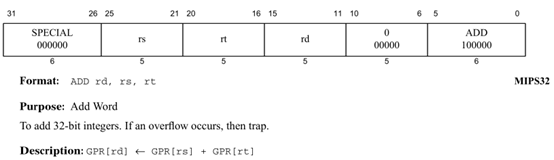
\includegraphics[width=\linewidth]{0.png}
    \caption{MIPS指令集下add指令详细格式}
    \label{FIG1}
\end{figure}

该指令是R-type指令,一共分为6部分。

除6-10位规定为0外,其余每一部分都需要通过译码电路单独提出来,因此译码电路的逻辑如下:
\begin{itemize}
\item 操作码optioncode取指令的31-26位;
\item 源寄存器rs的地址取指令的21-25位;
\item 源寄存器rt的地址取指令的16-20位;
\item 标寄存器rd的地址取指令的11-15位;
\item add的功能码取指令的0-5位;
\end{itemize}
根据以上阐述的add指令功能确定所需的数据通路。

add指令的功能是将源寄存器rs和rt两个内容相加,结果存入目标寄存器rd。
因此需要用到寄存器堆和ALU这两个部件。

首先根据rs和rt的地址从寄存器堆中取出相应的值,送到ALU进行运算,ALU再把运算结果返回寄存器堆,并写入地址为rd的寄存器中。
寄存器堆需要两个5位输入接受两个源寄存器的编号以及两个32位输出提供对应寄存器的值,还需要一个32位的输入接受来自ALU的运算结果以及一个5位输入接受目标寄存器的地址。

除此之外还需要时钟信号控制寄存器堆的写入与清零操作。

最后所有指令都需要先进行取指,因此都需要用到PC和nPC部件。
其中PC部件需要有32位输出提供指令的地址,需要有时钟信号保持PC在一个时钟周期内内容不变,
需要复位信号控制CPU在每次工作开始时PC的值都为0。
nPC部件负责计算下一条指令的地址,
可以使用组合逻辑实现,需要一个32位输入输出各一个。


   
beq指令和功能如下图所示:
​​\begin{figure}[H]
    \centering
    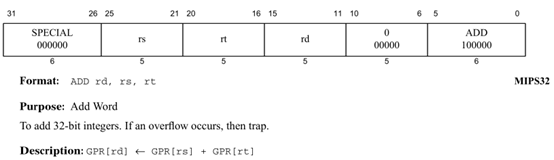
\includegraphics[width=\linewidth]{1.png}       
    \caption{MIPS指令集下beq指令详细格式}
    \label{FIG2}
\end{figure}

该指令有四部分,译码电路需要如下所示的接线:
\begin{itemize}
\item 操作码optioncode取指令的26-31位;
\item 源寄存器地址rs,rt分别取21-25,16-20位;
\item 跳转偏移量offset取0-15位;
\end{itemize}

beq指令的功能是当寄存器rs和rt内的值相等时,跳转到当前指令的偏移量offset处。
涉及到的部件有寄存器堆,ALU,NPC和Extend立即数拓展单元。

首先从寄存器堆中取出rs和rt的值,送到ALU进行比较(相减),若Zero信号为1则说明两个寄存器内的值相等,
nPC接收Zero信号并加offset(有符号扩展)从而产生下一条指令的地址。
所以需要添加的新信号是ALU的Zero信号用来判断两个数是否相等,nPC也要添加相应的输入,
添加32位输入接受来自经过Extend拓展后的立即数。

按照上面方法分析所有指令,分析完成后即可得到最终的单周期CPU的数据通路,如下:

\begin{figure}[H]
    \centering
    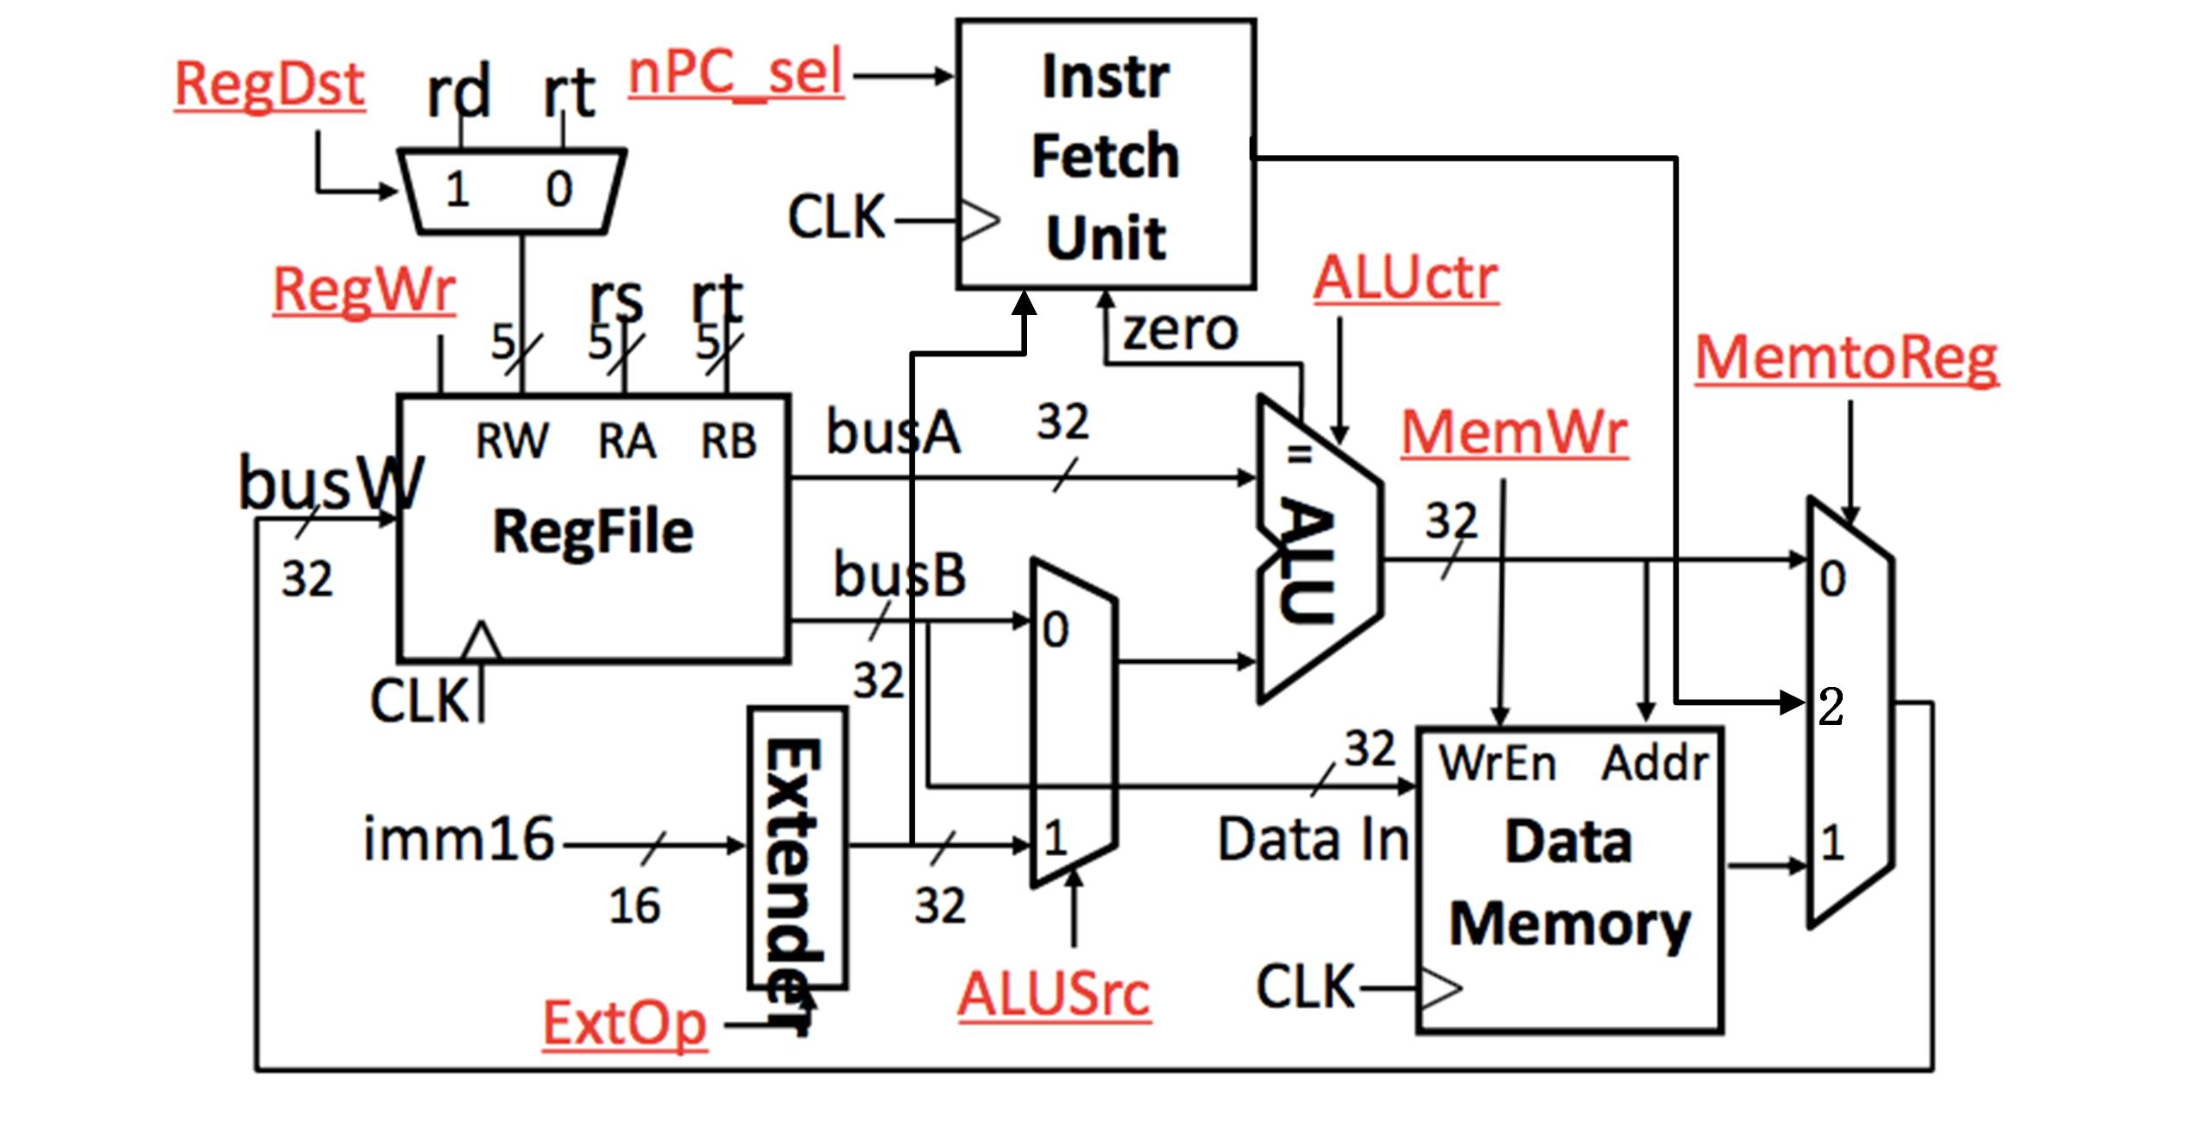
\includegraphics[width=\linewidth]{2.png}
    \caption{单周期CPU的数据通路(截取自老师提供的PPT)}
    \label{FIG3}
\end{figure}
​​
有了数据通路,下一步就是对控制器进行设计

\subsection{设计controller(用于控制各个模块的使用}

指令控制信号真值表如下
\begin{figure}[H]
    \centering
    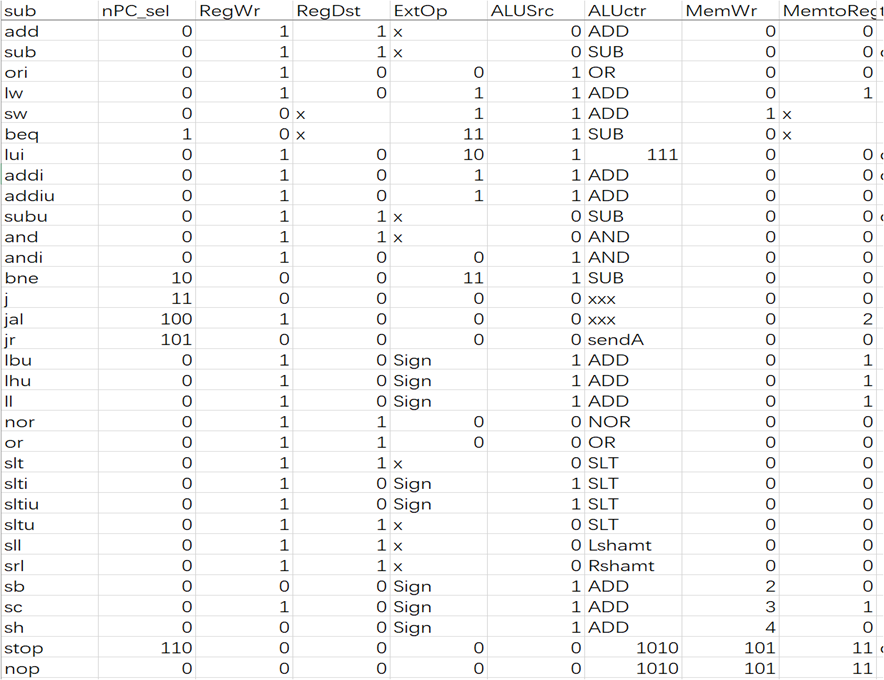
\includegraphics[width=\linewidth]{3.png}
    \caption{指令控制信号表}
    \label{FIG4}
\end{figure}​​

具体实现方式即与或门阵列,大致思路如下所示:
\begin{figure}[H]
    \centering
    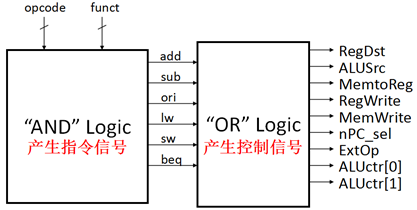
\includegraphics[width=\linewidth]{4.png}
    \caption{Controller的具体实现——与或门阵列}
    \label{FIG5}
\end{figure}

​​
\subsection{进行代码实现}
模块化实现代码,由顶层模块进行控制。
\begin{figure}[H]
    \centering
    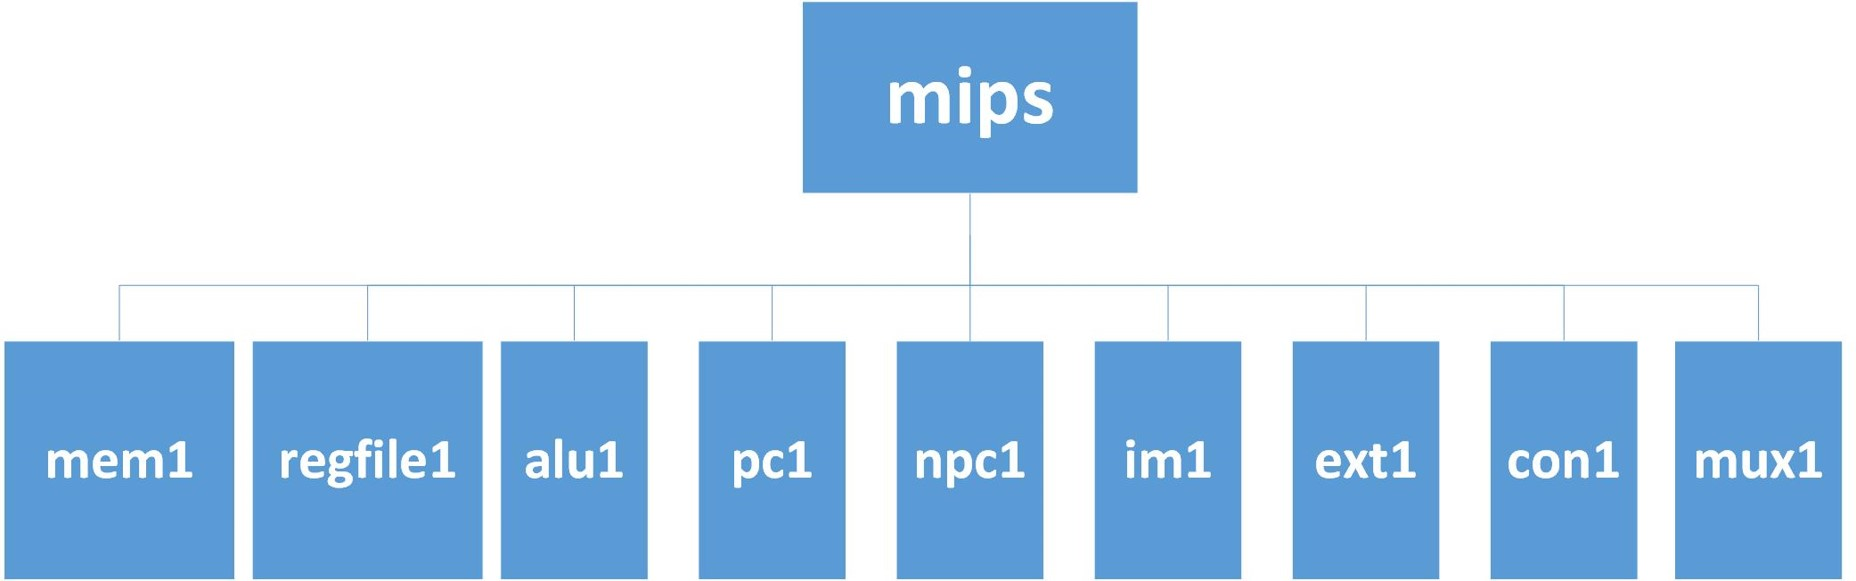
\includegraphics[width=\linewidth]{8.jpg}
    \caption{CPU模块}
    \label{FIG7}
\end{figure}

\subsection{测试}
通过载入并运行相应的汇编,查看相应寄存器或者数据内存的结果来验证该指令是否成功进行

\subsection{扩展指令集,并再次测试}
重复之前的操作

\subsection{运行高级语言的程序,通过数码管展示效果}

\begin{figure}[H]
    \centering
    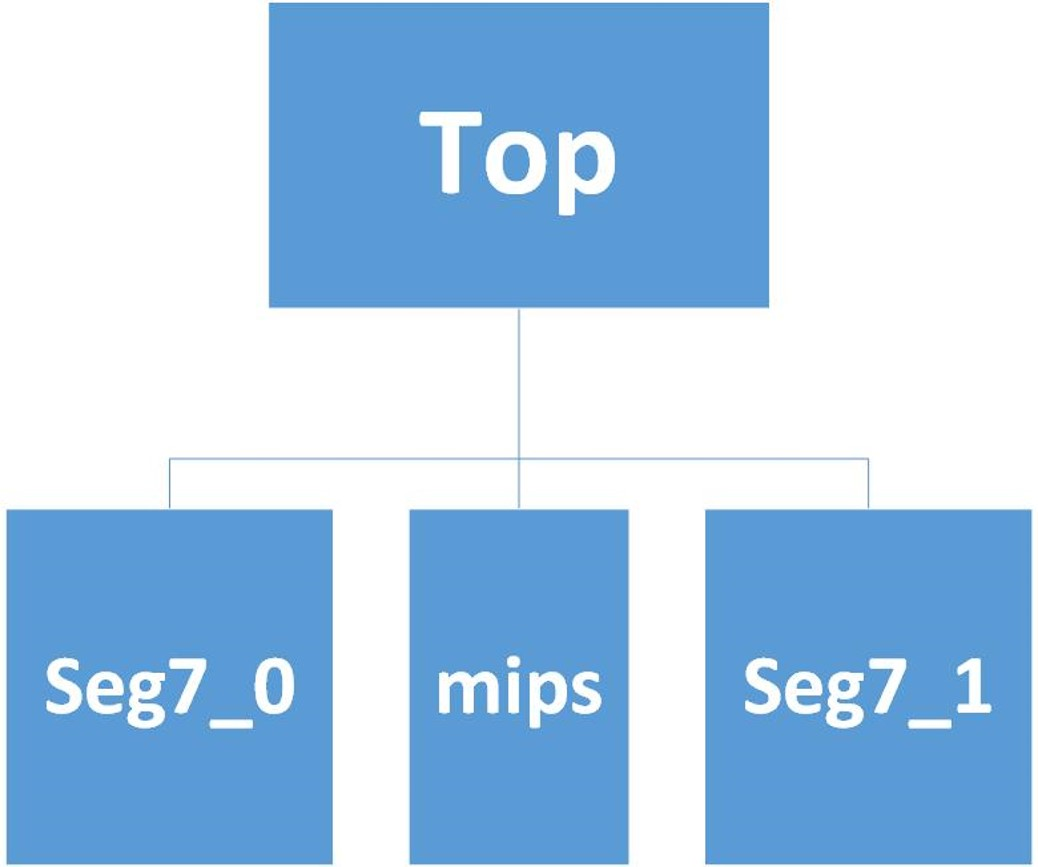
\includegraphics[width=\linewidth]{9.jpg}
    \caption{包括数码管的顶层模块}
    \label{FIG8}
\end{figure}

下文中介绍具体内容

\section{实验结果}

书写高级语言代码(本实验中为驱动数码管的斐波那契数列程序),并编译为mips平台下指令集,并针对机器码进行适当修改
\begin{figure}[H]
    \centering
    \subfigure[C语言]{
        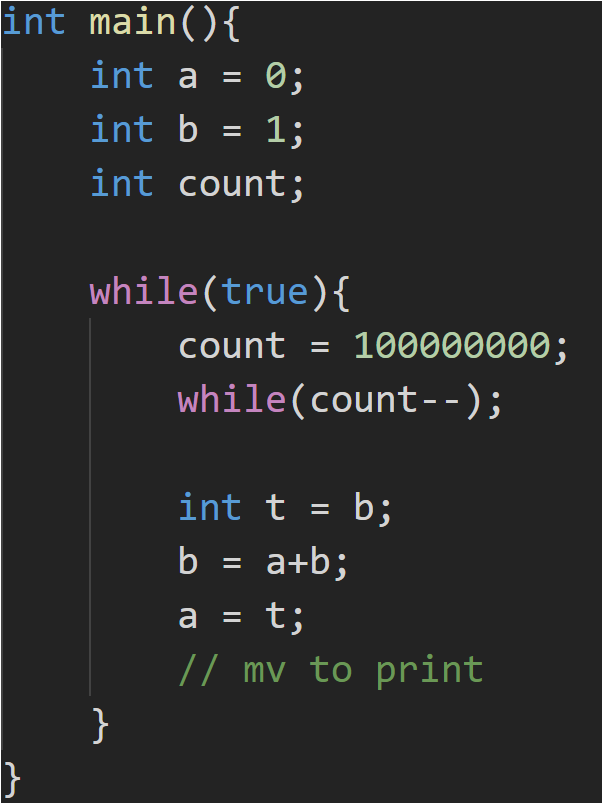
\includegraphics[width=0.3\textwidth]{5.png}
    }
    \subfigure[汇编]{
        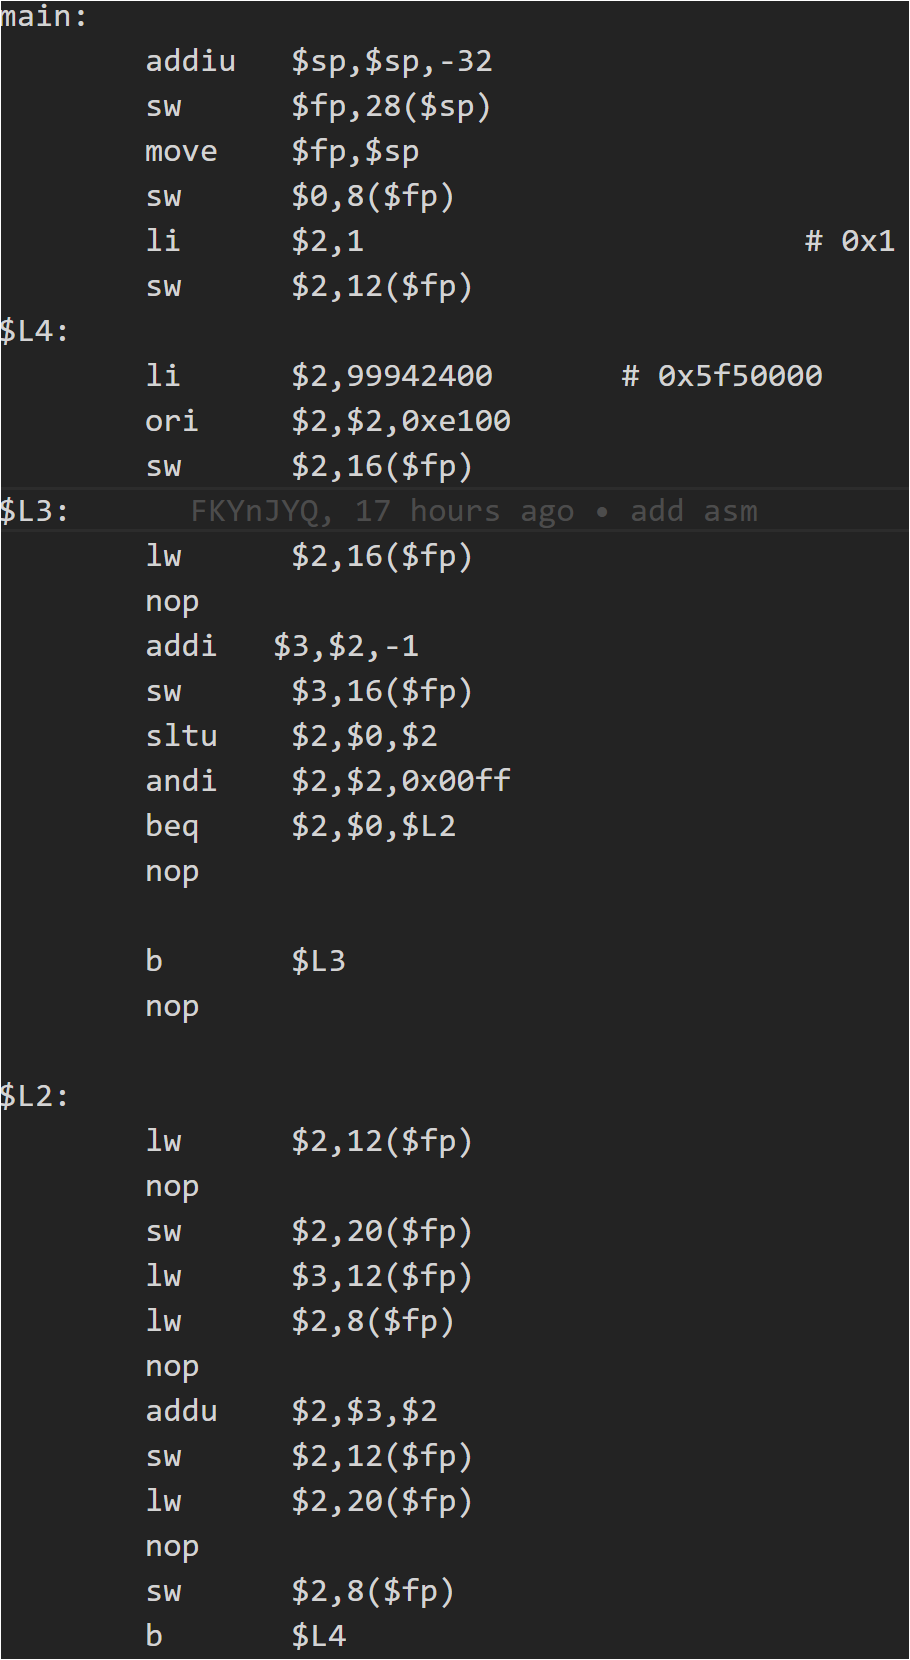
\includegraphics[width=0.3\textwidth]{6.png}
    }
    \subfigure[机器码]{
        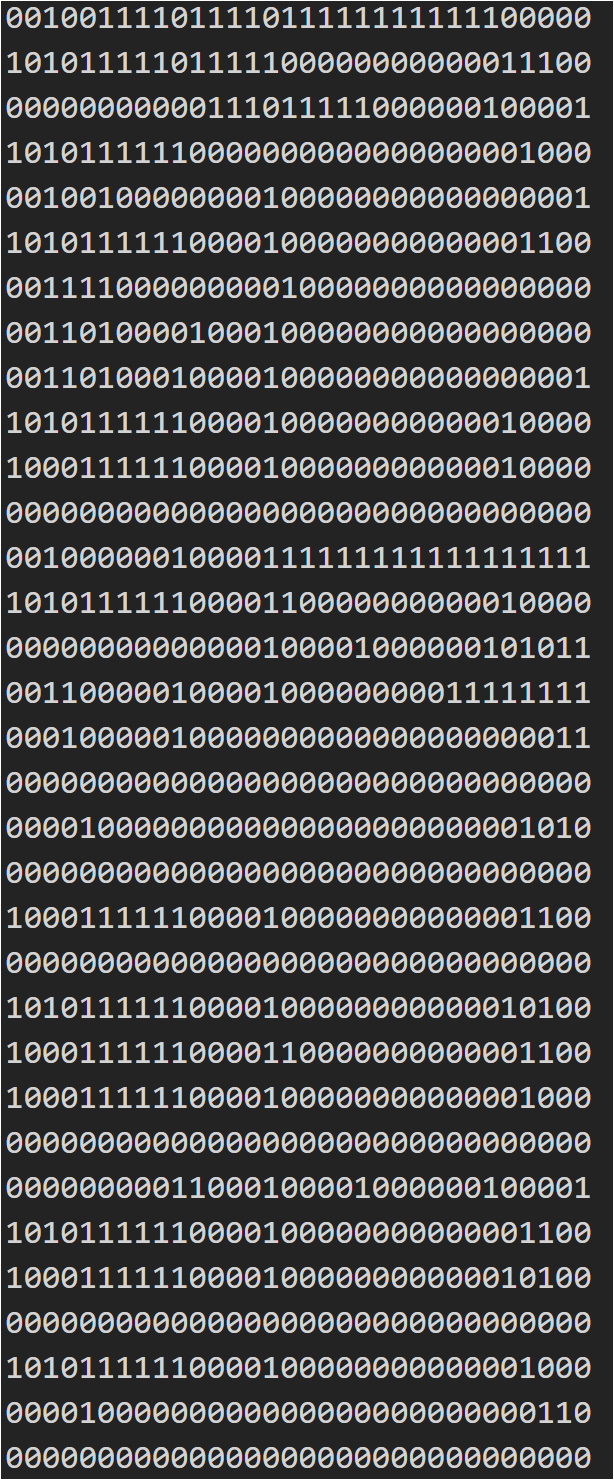
\includegraphics[width=0.3\textwidth]{7.png}
    }
    \caption{从C语言到MIPS架构下机器码}
    \label{FIG6}
\end{figure}
烧录并运行斐波那契数列程序,将结果展示在数码管上


\section{实验过程中问题的处理、讨论和改进思路,收获和体会}
\subsection{问题及问题解决办法}

\subsubsection{从C语言编译生成机器码后需要通过手动修改部分机器码来适应到我们的MIPS平台}
\begin{itemize}
    \item 有几个指令不匹配(addiu,nop,move)
    \item 编译结果默认IM与DM共享一段内存,但实际精简指令集计算机IM与DM有些情况下是分离的,会导致跳转指令有问题
\end{itemize}

\subsubsection{对只有输入或只有输出的模块(CPU模块只有Clk和Reset输入信号)进行implement时,综合工具会将其优化掉导致出现问题。}
      
解决办法:
添加输出并将输出传递给数码管驱动模块输入端

  
\subsubsection{变量名称容易混淆(协同开发的时候)}

\begin{itemize}
    \item warning非常重要
\item 要统一命名风格、甚至强制执行
\item 在利用其他编辑器编写代码后,回到vivado检查warning
  
\end{itemize}


\subsubsection{Device program之后,数码管始终为0}

是否是竞争问题?

我们逐一排查后,分析有可能是分频原因,在分频后(20倍时钟周期),解决了该问题,成功驱动数码管

\subsection{改进思路}
\subsubsection{从单周期到多周期}
  
难度较大(跟支持指令数成正比)。
我们进行了理论学习和分析,但由于代码工作量较大没有实现。
  
\subsubsection{支持浮点类型的指令集}
我们进行了IEEE 754 标准的学习,可以考虑下一步进行支持。
  
\subsubsection{驱动更多的外接设备}
由于时间原因,我们只驱动了数码管。
但是由于我们可以利用C语言进行控制,
因此增加外界设备的工作量会比纯Verilog小一些。
并且利用高级语言控制外接设备会更加方便。

\subsection{收获和体会}

\begin{itemize}
\item 了解了CPU的设计细节
\item 指令集的基本设计思想和作用
\item 汇编是如何实现高级语言的功能(高级语言到汇编到机器码到具体执行)
\item Verilog 的一些最佳实践
\item 模块化开发思想
\item 使用git进行vivado工程的版本控制
\item 快乐
\end{itemize}


\section{小组成员分工}
王聚海

\begin{itemize}
\item CPU组成的学习及CPU设计
\item 部分CPU功能模块的书写
\item CPU模块互联
\item 对汇编及机器码进行调试
\item 顶层top模块书写
\end{itemize}


冯开宇
\begin{itemize}
    \item CPU组成的学习及CPU设计
    \item 部分CPU功能模块的书写
    \item CPU指令集扩充
\item 汇编及机器码的生成
\item 对工程进行版本控制
\end{itemize}


刘思雨
\begin{itemize}
\item CPU组成的学习及CPU设计
\item 部分CPU功能模块的书写
\item 数码管驱动模块的书写
\item 顶层top模块书写
\item 相关资料收集
\end{itemize}

\section{参考资料}

\begin{itemize}
    \item 老师提供的两份PPT
    \item MIPS Reference Data
\end{itemize}

\section{项目地址}

\href{https://github.com/bit-logic-computer-design-2019/simple-cpu}{simple-cpu}

\end{document}